\chapter{An Introduction to Credit Derivatives}\label{chap:review}

The aims of this chapter are to provide the requisite
background to be able to understand how the key credit derivative instruments are used and priced. We survey many of the recently developed extensions to standard credit derivative pricing. We look at the introduction of default risk into option pricing \cite{JS1987}.
Credit Derivatives are financial securities that facilitate the transfer of credit risk from one agent to another. A periodic or upfront fee is paid by an agent in return for a structured payment should one of the underlying reference firms default.  Default can be outright bankruptcy or debt restructuring. Ratings data provided by the ratings agencies\footnote{Moody's KMV, S \& P, and Fitch amongst others} allows buyers and sellers to gauge the potential for either ratings changes or default.

\section{A Review of Credit Risk}\label{sec:cred_review}
\index{Credit Risk! Review}

\subsection{Model Risk}

Model Risk is the risk associated with using an inadequate model \cite{hs2002}. Model risk is amplified for CDOs as there can be errors in modeling both returns from entities and the relationships between entities \cite{bv2005}.  We also discuss the risks associated with Monte Carlo simulations in Appendix~\ref{subsec:accuracy}.

\subsection{What is Credit Risk?}\index{Credit Risk}

We begin with some definitions that will motivate credit based instruments.

\begin{definition}[Credit Risk]
\begin{rm}
is the risk due to uncertainty in a counterparty's ability to meet its obligations. Credit risk covers many different types of obligations from loans to complex derivative deals. 
\end{rm}
\end{definition}

\begin{definition}[Credit Risk Assessment]
\begin{rm}
Credit risk is assessed using the {\bf default probability}, {\bf credit exposure}, and {\bf recovery rate}. The default probability is the probability a counterparty will default its obligation, the credit exposure is the size of the outstanding obligations if a default occurs and the recovery rate is the fraction of the exposure that may be recovered through either post-default settlement or bankruptcy proceedings.
\end{rm}
\end{definition}

\begin{definition}[Correlation Risk]
\begin{rm}
Default correlation between two credits helps to determine the probability of both credits defaulting within a specified time horizon. The defaults of different obligors might be dependent on several fundamental factors. Direct links between two companies - for example, one obligor is a large creditor of the other, or one may own equity in the other - can cause their credit quality to be correlated. Firms within the same industry that are exposed to price shock to the same input factors or that depend on demand factors in the same markets could also be correlated. The general state of the economy in a region, country or industry also strongly influences the credit quality of otherwise unrelated debtors. Historically, we have seen that defaults tend to cluster, say, within an economic downturn.
\end{rm}
\end{definition}


\subsection{Credit Risk Models}

\cite{mer1974} introduced the first modern model of default which required adapting a
firms capital structure and default assumption to the Black-Scholes model where equity
is considered a call option on the firms assets. In this model a firm defaults if the asset value falls below a critical value attached to the value of the firm's liabilities. 


\subsubsection{Structural versus Reduced Form Models}

Credit Risk has been modeled using structural and reduced form models.
Merton's structural models provide a link between the probability of default and the firms 
fundamental financial variables, namely, assets and liabilities \cite{Eli2006}. \cite{mer1974} showed that stock could be viewed as a call option on the firm with the strike price equal to the face value of a single payment debt.
We can then obtain the default probability for the firm over one period and this can be repeated stepwise to obtain a hazard rate function, a function which provides the default probability of a firm over time. Default correlation may then be introduced by asserting that assets of different companies follow correlated processes. It is computationally expensive to build the risk analysis of a portfolio based on default correlation.  1000 obligors would require $\frac{(1000)^2 - 1000}{2}$ default correlations.

Reduced form models rely on market prices of the firms defaultable instruments to obtain default probabilities and credit risk dependencies. Therefore these models do not link credit risk and the firms assets and liabilities. They use a Poisson process approach, described in definition~\ref{def:poisson}, to model default times and are also computationally expensive \cite{ds1999}.


Vasicek introduced the Single Factor Model (1987,1991,2002). Simplifying assumptions
in this model \cite{Eli2006} are:
\begin{enumerate}
\item The correlation coefficient is the same for any two firms, see equation~\ref{eq:onefactor}.
\item We know the individual default probabilities of each firm defaulting at time $t$. Vasicek single factor model introduces dependence between models.
\item The default probabilities of all firms is the same.
\item The number of credits in a portfolio is very large such that as $N \to \infty$ allows for us to apply the law of large numbers.
\item The Loss Given Default is deterministic and the same for all firms.
\item The size of each credit in a portfolio is similar.
\end{enumerate}




\section{Pricing of Credit Derivatives}\index{Credit Derivative! Pricing}

\subsection{Risk Neutral Pricing \& Credit Default Swaps}\label{subsec:rnpricing}\index{Risk Neutral Pricing}

A Credit Default Swap (CDS) is a bilateral contract wherein the buyer of risk sells protection to insure the seller of risk (buyer of protection).  In the case of a credit event, i.e., default or possible rating downgrade, the seller of risk has the right to sell bonds of the affected issuer to the risk buyer.  Until maturity of the CDS, or default, whichever occurs first, the protection buyer must make periodic payments to the protection seller.  The CDS contract states whether settlement is physical delivery or cash upon default.

A CDS is priced using the term structure of default probabilities. In a risk neutral setting investors do not require an incentive to bear risk and so the price of an asset can be found by discounting the expected pay-offs with the risk free rate. Obviously the risk neutral probabilities must take into account risk aversion of investors and assign higher probabilities to 'bad' states.

A corporate bond may be priced at $P$ by incorparating the default probability and recovery rate in the expectation of a bond price \cite{lp2007}.  The recovery rate, $R$, where $0 \geq R \leq 1$, is the proportion of par that a bond will trade at after a default event occurs. In the following $M$ is the notional, $CF$ is the cashflow received at time $t$, $PD^0_t$ is the probability of default in $t$ from today and $r_t$ is the risk free spot rate.


\begin{align}
 P = E \left[ \sum^T_{t = 1} \frac{CF_t}{(1+r_t)^t} \right] = \frac{M (1 - PD^0_1) + M.R.PD^0_1}{1+r} \nonumber
\end{align}

This formula, which shows that the expected price can be in two different states, can be rearranged such that the difference between a risk free bond, $B_0$, and a risky one with the same cash flows is the discounted expected loss from holding the risky over the risk-free bond.
We sum over all default dates $\tau$ until maturity $T$. $C_\tau$ is the claim bondholders have at default.

\begin{align}
 B_0 - P = \frac{PD^0_1(M - M.R)}{1+r} = \sum_\tau PD^0_\tau \left( B^\tau_0 - \frac{C_\tau. R }{(1 + r_\tau)^\tau } \right) \nonumber
\end{align} 

A CDS is priced by comparing the expected payoffs of the buyer and seller of protection. For an annual percentage fee $s$ the expected payments made by the buyer of protection are
\begin{align}
E \left[ fee \right] = \frac{M * s}{freq \sum_\tau \left[ \frac{1 - \sum_{t=1}^{\tau-1} PD^0_\tau }{(1 + r_\tau)^\tau } \right]}
\end{align} 
where $PD^0_t$ is the probability of default in $t$ from today.  The expected payments in the event of default are
\begin{align}
E \left[ default payments \right] = M \sum_\tau ( 1 - R - A(\tau) R) \frac{PD^0_\tau}{(1 + r_\tau)^\tau}
\end{align} 
where $A(\tau)$ is the accrued interest determined from coupon rates and payments.  So both parties must settle on a CDS contract such that the spread $s$ equates $E[fee]$ and $E[default payments]$ at a given recovery rate $R$. This is the fair price of a CDS and is expanded upon in {\cite{cs2003,jt1995,Amm2002,Schm2003}}.

\subsection{Copula Functions}\index{Copula Functions! Introduction}\index{Copula Functions! Gaussian}

The Structural and Reduced form models are both computationally time consuming; hence the Gaussian copula model has become the de facto market standard. This was introduced by \cite{Li2000}.  Essentially, in a copula model the joint probability distribution for the default times of multiple companies is constructed from marginal distributions to create a simple multivariate joint distribution \cite{hw2004}. Figure~\ref{fig:copula} shows a Gaussian Copula for correlation of 0.7.

To introduce copula functions we note that a standard Monte Carlo simulation, say, of random returns, requires selection of a uniform random number $u_i$ in the range (0,1) and this is then inverted with the cumulative distribution function to get $r_i = F^{-1}_i (u_i)$ \cite{SM2005} which has the distribution function $F$.  In a multivariate setting the joint distribution of $n$ random variables $X_1, X_2, ..., X_n$ is:

\begin{align}
F(x) = P[X_1 \leq x_1, X_2 \leq x_2, ..., X_n \leq x_n]  \nonumber
\end{align}

So we know that we can calculate the marginals from $F^{-1}_i (u_i)$ and if $F(r_1, r_2, ..., r_n)$ represents a multivariate distribution it will have a unique Copula representation:
\begin{align}
F(r_1, r_2, ..., r_n) = C( F_1, F_2, ..., F_n) \nonumber
\end{align}

\begin{figure}
\centerline{\scalebox{0.5}{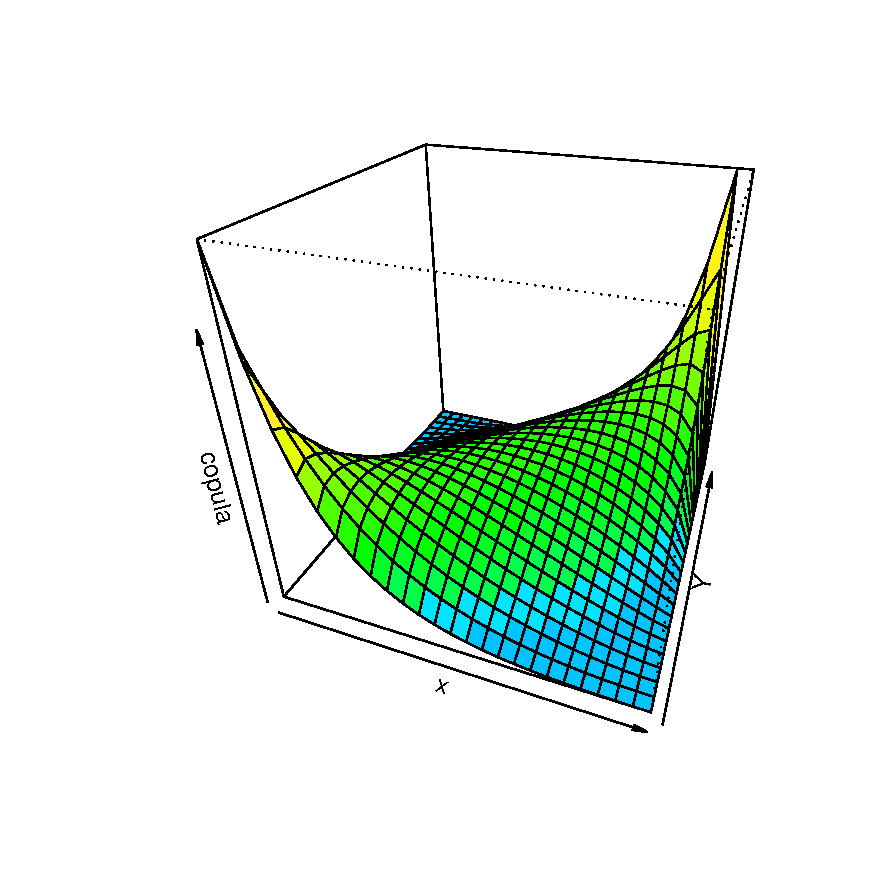
\includegraphics{pictures/Copula.pdf}}}
\caption{\label{fig:copula}A Two-dimensional Gaussian copula}
\end{figure}

This is known as Sklar's theorem \index{Sklar's Theorem} where $C$ is the distribution function of $F$ which shows that the dependence structure can be completely characterised by copula function $C$. This can easily be applied to the default probabilities of obligors within CDOs. Copula functions are extensively described in \cite{nel2005,Sch2003}. There are many copula functions many of which provide better fits for CDO pricing than the Gaussian copula. \cite{hw2004} presents the Double-t and \cite{Sch2003} surveys other copulae which provide alternative default dependence structures.

\subsection{First to default instruments}
\index{FTDs}
\index{First to default}

A First to Default (FTD) basket swap extends CDSs to cover the credit risk for a portfolio of reference entities.  The protection buyer pays a periodic fee of $s$ to the protection seller until either default or maturity of the FTD is reached.  The FTD is terminated after the first default event of any of the reference entities and default payment is then 1-R of the defaulted entity. A typical FTD basket may contain between 4 and 12 reference entities. If the probability of multiple defaults is low then the basket should be well protected by an FTD \cite{Sch2003}. 

FTDs are useful instruments to each side of the FTD contract.  The buyer of protection is able to protect a whole basket of entities at a cheaper cost than purchasing individual default protection and the seller has limited his exposure to one default, his premium for this has increased and the only downside is that the risk of a default payment has increased.
As the size of the basket increases protection given by an FTD weakens and so { \em First Loss Structures } are commonly used.  We do not consider these further though they are detailed in \cite{Sch2003}.

\subsection{$N^{th}$ to default instruments}\label{subsec:NTDs}
\index{NTDs}
\index{N to default}

An $N^{th}$ to default basket swap only differs from an FTD in the specification of the default event, this now being the $n^{th}$ and not the first default event. The valuation of an NTD is based on the probability that the $n^{th}$ default will occur between $T_1$ and $T_2$ as opposed to a standard CDS whose valuation is simply based on default occurring between $T_1$ and $T_2$.  When the $n^{th}$ default occurs the seller pays the notional times $1-R$ and the buyer must pay any accrued payment required to cover the elapsed time since the previous payment.  If we consider a basket of we require application of a Poisson process to generate default probabilities.


\begin{definition}[Poisson Process]\label{def:poisson}\index{Poisson Process}
\begin{rm}
A Poisson process with intensity $\lambda > 0$ is a non-decreasing integer value process with initial value $N(0) = 0$ with independent increments that satisfy, for all $0 \geq t \leq T$
\[
	P[N(T) - N(t) = n] = \frac{1}{n!} (T-t)^n \lambda^n e^{-(T-t)\lambda}
\] 
such that $P(0,T) = e^{-\lambda T}$.  Poisson processes are commonly used within jump diffusion models.
\end{rm}
\end{definition}

The default probabilities within a basket of $n$ entities are generated by Poisson processes with a constant default intensity $\lambda_i$ where $1 \geq i \leq n$, such that
\[
	PS_i(t) = e^{-\lambda T} \quad \mbox{and} \quad PD_i(t) = 1 - e^{-\lambda T}
\]
where $PD_i(t)$ is the risk neutral probability that entity $i$ will default before time $t$ \cite{hw2004}.


Basket Default Swap pricing generally utilises Monte Carlo simulation techniques though in Section~\ref{sec:ntd_surface} we chose to implement the approach presented in \cite{hw2004};
this is a simple process which requires the probability distribution of the number of defaults by a time $T$. This paper also derives a recurrence relationship for the fast computation of this which we implement. \cite{cg2008} present an importance-sampling technique which forces all paths to produce at least $n$ defaults in pricing an
NTD; this increases the probability that the next asset defaults prior to maturity until
$n$ defaults have occurred and requires adjusting the distribution of risk factors to provide more relevent scenarios.\\

The risk neutral pricing of an NTD (where expectations are taken under risk neutral measures) is computed by equating the expected value of the discounted premium payment leg with the expected value of the discounted default leg. In the following, following \cite{Gal03}, $k$ is the seniority of the NTD, $\Delta$ is the time interval between premiums,  $B(0,t_i)$ is the risk free discount factor over interval $(0,t_i)$ and $M$ is the notional. For the premium leg:
\begin{eqnarray}\label{ntd_pl}
 PL & = & E \left[ \sum_{i=1}^n s M \Delta B(0,t_i) 1_{\{\tau_k \leq t\}} \right] \nonumber\\
 & =	& \sum_{i=1}^n s M \Delta B(0,t_i) 1 - F_{k} (t_i) \quad\mbox{where}\quad F_{k} (t_i) = P(\tau_k \leq t)
\end{eqnarray}

and the default leg (DL) is the default premium (DP) less the accrued premium (AP) where
\begin{eqnarray}\label{ntd_dp}
 DP & = &  E \left[M \sum_{i=1}^n (1-R_k) B(0,t_i) 1_{(\tau_k \leq t)} \right] \nonumber\\
 & = &	M \sum_{i=1}^n (1-R_k) \int^T_0 B(0,t_i) F_k dt
\end{eqnarray} 
and
\begin{eqnarray}\label{ntd_ap}
 AP & = & E \left[M \left( s \frac{T_k - t_{i-1}}{t_i - t_{i-1}}  \Delta \right) B(0,\tau_k) 1_{\{t_{i-1} < \tau_k \leq t_i\}} \right] \nonumber\\
&  = & s M \sum_{i=1}^n \int^t_{t-1} \frac{u - t_{i-1}}{t_i - t_{i-1}} \Delta B(0,u) F_k du
\end{eqnarray} 

We can now price the NTD such that s is the fair spread which ensures that PL - DL = 0 to get

\begin{align}\label{ntd_ap}
 s = \frac{ \sum_{i=1}^n (1-R_k) \int_0^T B(0,t_i) F^{kth = j}_k (dt)   }{\sum_{i=1}^n \Delta B(0,t_i) 1 - F_{k} (t_i) + \int^t_{t-1} \frac{u - t_{i-1}}{t_i - t_{i-1}} \Delta B(0,u) F_k du}
\end{align} 

Further detail on pricing NTDs is presented within \cite{Sch2003,Gal03}.

\subsection{Collateralized Debt Obligations}

Collateralized Debt Obligations (CDOs) can be either cash CDOs which consist of credits, debts or loans or synthetic CDOs which can be a portfolio of CDSs. In Figure~\ref{fig:cdostructure} we see an overview of the structure of a CDO instrument. Pricing for CDOs has been widely analysed in \cite{Neu2007,LBG2008}. As with other derivative instruments a CDO consists of fixed and floating legs, $X_F$ and $X_V$, respectively where you receive $X_F$ and pay $X_V$ and the premium is chosen such that $X_F = X_V$.

CDOs are divided into a tranche structure $[K_L,K_U]$ where $K_L$ is the attachment point and $K_U$ is the detachment point. Each tranche is fixed such that the NPV of cashflows paid is zero. Holders of tranche $[K_L,K_U]$ have limited their loss exposure to $K_U - K_L \% $ of the initial portfolio value. Losses are paid by tranche holders during the life of a CDO with a predetermined frequency.  Holders of a tranche $j$ with $[K_L,K_U]$  receive periodic payment with frequency $\nu$, usually 0.25 years, equal to a premium $s_j$ of the outstanding notional of the tranche. Loss $L_{t,j} = min (L_t,K_U) - min (L_t,K_L)$ is a percentage of total portfolio loss.  The structure of cash flows for tranche $j$ holders at each payment date receive $X_F$ and pay $X_V$ where
$ X_F = s_j \nu \Gamma_{j,t} $ and 
$	X_V = (Z_{j,t}-Z_{j,t-\nu})M  $ for $t = \nu, 2\nu, \ldots, T$ and $s_j$ fixed and $\Gamma_{j,t}$ is the outstanding notional, a decreasing function of portfolio losses and total portfolio loss is $L_t M$.   The outstanding notional is given by
\begin{align}
\Gamma_{j,t} = \begin{cases} 
						(K_U-K_L)M & L_t < K_L \nonumber \\
						(K_U-L_t)M & K_L \leq L_t \leq K_U  \\
						0			& L_t \geq K_U 
				\end{cases}
\end{align}


In these products the originator may retain the equity tranche to show that the issuing bank knows best the riskiness of the credits and that it holds the riskiest tranche is a clear signal that this is a fair deal to enter into.


\begin{figure}
\centerline{\scalebox{0.8}{\includegraphics[viewport = 107 510 497 786]{pictures/CDOStructure.pdf}}}
\caption{\label{fig:cdostructure}The Structure of a CDO}
\end{figure}


\subsection{LHP One Factor Gaussian Copula CDO Pricing}

Assumptions of the Large Homogenous Portfolio (LHP) \cite{lp2007} are:
\begin{enumerate}
\item The reference portfolio is homogenous so all assets share the same pairwise correlation, default probabilities and recovery rates.
\item The number of assets in the portfolio tends to infinity.
\item The default dependency structure is based on a Gaussian Copula model.
\item Each tranche is priced on a single flat correlation, the compound correlation of the tranche.
\end{enumerate}

Default of each obligor is condtionally independent given a level of state risk $M$ and occurs if  $X_i = \sqrt{ \rho } M + \sqrt{ 1 - \rho } \epsilon_i$ is less that a threshold where $M$ and $\epsilon_i$ are independent normal variables.

The LHP Gaussian Copula models the default correlation using a firm value approach.  We begin by modeling the default dependency structure assuming all assets are correlated with a single market variable, following the formulation of \cite{Sch2003}:
\begin{align}\label{eq:onefactor}
X_j(T) = \sqrt(\rho) Z + \sqrt(1-\rho) \epsilon_j		\quad	\forall_j = 1, 2, \ldots, n
\end{align}
where $cov(\epsilon_i, \epsilon_j) = 0$ for $i \neq j$ and $cov(Z,\epsilon_i) = 0$ for all $i$.
$\rho$ is the correlation of asset values with the market factor M. $\epsilon_j$ is the idiosyncratic firm specific risk.  This process is similar to the CAPM (Capital Asset Pricing Model) formulation of splitting risk into two components.  As we assume that M and all $\epsilon_j$'s are normal this is the gaussian copula model.

$X_j(T)$ is the value of a firm $j$'s assets at time $T$. When $X_j(T)< K(T)$ where
$K(T)$ is our default barrier the firm experiences default.  Applying~\eqref{eq:onefactor} into this and rearranging for idiosyncratic risk gives us:
\begin{align}\label{eq:epFactor}
\epsilon_j \leq \frac{K(T) - \sqrt(\rho)M}{\sqrt(1-\rho)}
\end{align}

Now we seek the probability of default conditional on $M$:
\begin{eqnarray}
 p_j(t,T \mid M) & = & Prob[X_j(T)< K(T)\mid M] \nonumber\\
 & = & Prob[\epsilon_j \leq \frac{K(T) - \sqrt(\rho)M}{\sqrt(1-\rho)} \mid M ]  \nonumber\\ 
 & = & \phi \left( \frac{K(T) - \sqrt(\rho)M}{\sqrt(1-\rho)} \right) \nonumber \\
& = & \phi \left( \frac{\Phi^{-1}(1 - e^{-s(T-t)}) - \sqrt(\rho)M}{\sqrt(1-\rho)} \right)
\end{eqnarray}

We can now apply the important large portfolio assumption and assume that the number of defaulted credits is provided by the individual default probabilities conditional on $M$.  The loss fraction makes use of the recovery rate
\begin{align}
l_{pf}(t,T \mid M) = (1-R)  p_j(t,T \mid M)
\end{align}
and from this we can derive the payoff of a particular tranche condtional on $M$.  The unconditional loss, where the integral removes the dependency on $M$, is:
\begin{align}
EL^b_a(t,T_i,\rho ,s,R) = \int^\infty_{-\infty} Payoff\left[ a,b,l_{pf}(t,T \mid M) \right] \psi(M) dM \nonumber \\
= \int_{-\infty}^\infty \frac{1}{b-a}\left[ (l_{pf}(t,T \mid M)-a,0)^+ - (l_{pf}(t,T \mid M)-b,0)^+ \right] \psi(M) dM
\end{align}

This can be solved with numerical integration.  Losses start to erode the capital on a tranche only when all subordinate tranches are wiped out. \cite{HPW2005} show that correlation is positively dependent on default probabilities.




\subsection{Valuing a CDO swap}\index{CDO! Swap}

The price of a CDO swap is given by the following expression (further detail in \cite{Eli2006}):
%%\begin{equation}
\begin{eqnarray}
 V_{CDO}(0) & =  & E\left(\int^{T}_{0} \mathrm{e}^{- \int^t_0 r(u) du } dL_{[K_L,K_U]} (t) \right) \nonumber\\ 
& & - c E\left(\sum^{Q}_{i = 1} \mathrm{e}^{- \int^t_0 r(u) du } \delta_i \frac{(N_{[K_L,K_U]}(T_i) + N_{[K_L,K_U]}(T_{i-1}))}{2}  \right) \nonumber\\  
 & = & E\left(\int^{T}_{0} \mathrm{e}^{- \int^t_0 r(u) du } dL_{[K_L,K_U]} (t) \right) - c A_{[K_L,K_U]}(0)
\end{eqnarray}

where $A_{[K_L,K_U]}$ is the price of a risky annuity. Hence the breakeven spread, the coupon $c$ value which
ensures that the fixed and floating legs have the same value, is:

\begin{align}\label{credSpread}
 c_{BE}(0) = \frac{E\left(\int^{T}_{0} \mathrm{e}^{- \int^t_0 r(u) du } dL_{[K_L,K_U]} (t) \right) }{ A_{[K_L,K_U]}(0)}
\end{align}



%%\end{equation}

\subsection{Monte Carlo CDO Pricing}\index{CDO! Pricing}

Much work on pricing CDOs uses Monte Carlo simulations as any forward-rate based model has a very large state space.  An unbiased estimator will be generated to approximate the {\em true} price of a CDO.  As each trial is independent we can apply the central limit theorem which tells us that our difference between the true value and the simulation value is normally distributed with zero mean so we can approximate the sample standard deviation and from this we can form confidence intervals. More trials can be conducted it we then want to increase the simulation accuracy.  Monte Carlo processes are fully examined in \cite{Sch2003}.
\cite{hw2004} also present a useful methodology for pricing CDOs without Monte Carlo simulation.

\subsubsection{Multi-factor models}

The random variables defined in equation~\ref{eq:onefactor} can be extended to many factors with the following change
\begin{align}\label{eq:multifactor}
V_j(T) = \sqrt(\rho_1) M_1 + \ldots + \sqrt(\rho_n) M_n + \sqrt(1-\rho_1 - \ldots - \rho_n ) \epsilon_j			\forall_j = 1, 2, \ldots, n
\end{align}
such that the $M_i$ have independent distributions with zero mean and unit variance.  An example of the requirement for such a model might be within a global portfolio where there are stong intra-country correlations or if there are sector links within a portfolio. This models are covered within \cite{hw2004,Schm2003}.


\subsubsection{Student-t Copula Functions}

The Gaussian Copula one factor model is still considered the industry standard for CDO pricing \cite{Eli2006} but many other alternatives have been considered including the Double-t Copula \cite{hw2004} and the normal inverse gaussian \cite{Neu2007}, the latter of which we do not consider further.  The Double-t Copula essentially replaces the Gaussian one-factor model with one that is t-distributed on both systematic and idiosyncratic risk. The t-distribution should increase the more extreme values for the assets and so increase the probability of observing more defaults.


\subsection{Success of CDOs}\index{CDO! Success of}

The iTraxx and CDX indices of CDS on 125
names can themselves be structured and traded like a traditional synthetic CDO with
equity, mezzanine, and senior tranches. Like in a traditional CDO, the
standard tranches of CDS indices provide claims to the cash flows of the iTraxx CDS
portfolio, in return for payments by the investors if a default occurs within their tranche. 

CDOs have been immensely successful in the marketplace for many reasons including potential for spread arbitrage opportunities, the transfer of risk and, as noted in \cite{Gib2004}, that tranche sensitivities can be linked in to the business cycle.


\subsection{Single Tranche Trading}\index{CDO! Single Tranche Trading}

iTraxx tranches (or the iTraxx index itself) can also be used by
arrangers for the dynamic hedging of single-tranche CDOs. Single tranche traders have historically focussed on the mezzanine tranche so they may be riskier as they are unlikely to be fully hedged.

\subsection{Random Recovery Rates and Random Factor Loading}

\cite{as2005,Neu2007} present extensions to the form factor model shown in equation~\eqref{eq:onefactor} based on random factor loading. An example is the two point loading of \cite{as2005} where $X_j(T) = a_{ij}(Z) Z + v_j \epsilon_j + m_i$ 
\begin{align}
a_{ij} \left(Z_j \right) =  \begin{cases} 
						\alpha_{ij} & Z_j \leq \theta_{ij} \nonumber\\
						\beta_{ij} & Z_j > \theta_{ij}  
					 \end{cases}
\end{align}
and $\alpha_{ij},\beta_{ij}$ are positive constants and $\theta_{ij} \in \mathbb{R} $.  This can be viewed as a switching model where loading takes values $\alpha_{ij}$ with probability $\phi(\theta_{ij})$ and  $\beta_{ij}$ with probability $1-\phi(\theta_{ij})$ so if $\alpha_{ij} > \beta_{ij}$ then the factor loadings will decrease in $Z_j$. As the random factor model changes the correlation through factor exposure as a function of the factor itself this could represent asset values coupling more strongly to a poor economy.

\medskip
Despite the standard models assuming a standard recovery of 40\% research has shown these actually vary with credit event (i.e. default,rating up/downgrades). \cite{as2005} allow recovery rates to have both an idiosyncratic and a systematic risk factor.  Recovery rates are specified as $R = \phi(\mu_i + \gamma_i V + \sigma_{\epsilon_i} \epsilon_i)$. \cite{kre2008} extends this letting the recovery rate have a default triggering factor. In this model each obligor has a discrete recovery distribution noting that the average recovery rate must equal the quoted recovery rate so that consistency with the single name CDS market is maintained.  This model applies in scenarios where standard base correlation fails such as when spreads widened in March 2008 and senior tranches could not be priced. \cite{AH2008} present a similar extension.


\section{Implied Correlation}\index{CDO! Implied Correlation}\index{Implied Correlation}

The Black-Scholes model for pricing options presents a formula where the option price is a function of rate, time to maturity, underlying stock price and stock price volatility. When we have a market price of the option we can infer the volatility. This is the {\em implied volatility }. With the advent of the credit indices we can infer the default correlation coefficient from the given market spread.  Increasing maturities of CDOs will also lead to the generation of a forward correlation curve.


\begin{definition}[Volatility Smile]
\begin{rm}
The pattern that at-the-money options have a lower volatility than other options. The volatility smile will generally be calculated for vanila options and will then be used for more complex option modeling.
\end{rm}
\end{definition}

\subsection{The Implied Correlation Curve and the Credit Indices}

Given the market price of a single tranche CDO, the Vasicek Single Factor model and the default correlation coefficient $\rho$ we can compute $\rho$ which matches the price of a CDO.  For each tranche we can compute the implied default correlation.  This presents us with the problem of the { \em correlation smile }, where the spread for mezzanine tranches is lower than that of the equity and senior tranches.  Mezzanine tranche premiums are non-monotonic which unfortunately provides us with non-unique tranche premiums. If the pricing mechanism of equation~\eqref{credSpread} were correct there would be no { \em correlation smile}. We present a generated smile for iTraxx data for 31 July 2008 in figure~\ref{fig:impCorr}.

\begin{figure}
\centerline{\scalebox{0.5}{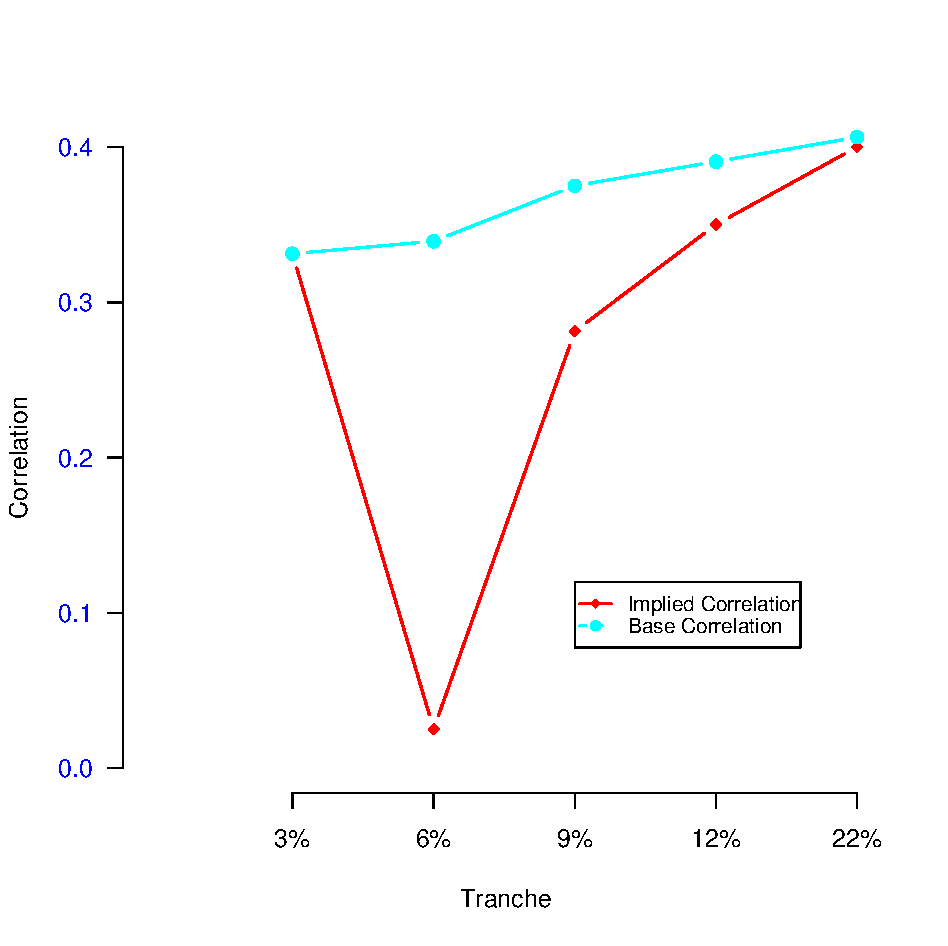
\includegraphics{pictures/impliedCorr.pdf}}}
\caption{\label{fig:impCorr}iTraxx EU S9 Implied and Base Correlation for 31 July 2008}
\end{figure}

Reasons for the correlation smile, collated in \cite{Eli2006}, include:
\begin{enumerate}
\item Different investor groups purchase different tranches and, hence, may have different views on correlations
\item Unknowns in correlation models affecting equity tranches, which are more sensitive to correlations, which may contain a model risk premium embedded in their prices
\item Variations in local demand conditions in prices
\item Disparities between different pricing models
\end{enumerate}

The implied correlation issue is still a contentious area within credit risk.  As noted in \cite{risk2006}, implied volatility can be assessed historically but it is far more difficult to view historical time to default correlations.

\subsection{Base Correlation Pricing Mechanisms}

Base correlation, introduced by \cite{MA2004}, uses the guaranted monotonicity of the equity tranche and proceeds to construct fictitious equity tranches which are used to construct mezzanine and subsequently senior tranches. This recursive { \em bootstrapping } technique relies on applying the implied correlation from the previous tranche.

Base correlation replaces implied correlation on the standard tranches with virtual tranches which all have the same lower attachment point of 0\%. So the set of virtual tranches contains $0 - K_U\%$ where the detachment point in $K_U \in { 3,6,9,12,22 }$. Any tranche can then have its loss decomposed into two tranches which have a $0\%$ detachment point to give us:-
\begin{align}
E(L[0,K_j])=E(L[0,K_{j-1}]) + E(L[K_{j-1},K_{j}])
\end{align}

Base Correlation allows for non-standard tranches to be easily priced and interpolated.
\cite{pw2007} show that extrapolation can be dangerous outside this and lead to arbitrage opportunities. 

Base Correlation is generated using the following bootstrapping process \cite{KL2004}:-
\begin{enumerate}
\item	Find the Equity Tranche Implied Correlation as for the standard compound correlation process. This requires solving for $0 = PV(0,K_1,S_{0,K_1},\rho_{K_1})$	
\item	For the next tranche we solve for $0 = PV(0,K_2,S_{K_0,K_1},\rho_{K_2}) - PV(0,K_1,S_{K_1,K_2},\rho_{K_1})$.  Note that the second term here uses $\rho_{K_1}$ from the previous step so we still have one equation with one unknown.	
\item	Iteratively apply step 2 to higher tranches.
\end{enumerate}

Base Correlation produces a correlation skew as shown in figure~\ref{fig:impCorr}. Each tranche is base correlation pricing is considered an equity tranche which is long correlation so all tranche PVs are increasing functions of the upper attachment point.
There is much debate as to whether base correlation is a suitable model or simply a process to remove the correlation smile. \cite{risk2006} notes that it is not arbitrage free, does not consider invidual spreads and all credits are equally weighted. In Spring 2008 the index spreads for senior tranches widened and base correlation methods failed \cite{kre2008}\footnote{and personal experience within Credit Risk IT!}. \cite{KL2004} presented scenarios where this would occur when the junior mezzanine tranche spreads were high which is what occurred in 2008 as these high spreads inverted the initial curve making it impossible to price senior tranches.




